%% ----------------------------------------------------------------
%% Thesis.tex -- MAIN FILE (the one that you compile with LaTeX)
%% ---------------------------------------------------------------- 

% Set up the document
\documentclass[a4paper, 11pt, spanish, oneside]{Thesis}  % Use the "Thesis" style, based on the ECS Thesis style by Steve Gunn
\graphicspath{Figures/}  % Location of the graphics files (set up for graphics to be in PDF format)

% Include any extra LaTeX packages required
\usepackage[square, numbers, comma, sort&compress]{natbib}  % Use the "Natbib" style for the references in the Bibliography
\usepackage{verbatim}  % Needed for the "comment" environment to make LaTeX comments
\usepackage{vector}  % Allows "\bvec{}" and "\buvec{}" for "blackboard" style bold vectors in maths
\hypersetup{urlcolor=blue, colorlinks=true}  % Colours hyperlinks in blue, but this can be distracting if there are many links.
\usepackage[T1]{fontenc}
\usepackage{selinput}
\usepackage{minted}
\SelectInputMappings{%
  aacute={�},
  ntilde={�},
  Euro={�}
}
\usepackage{babel}
\usepackage{csquotes}
\usepackage{titlesec}
\usepackage{graphicx}
\newcommand*{\justifyheading}{\raggedright}
\titleformat{\chapter}{\normalfont\huge\bfseries\justifyheading}{}{0em}{\bf\LARGE}


%% ----------------------------------------------------------------
\begin{document}
\frontmatter      % Begin Roman style (i, ii, iii, iv...) page numbering

% Set up the Title Page
\title  {Prototipo de Plataforma Estructurada para el Acceso a Sistemas de Transparencia Gubernamental}
\authors  {Esperanza Citlali Garc�a Medina}
\addresses  {\groupname\\\deptname\\\univname}  % Do not change this here, instead these must be set in the "Thesis.cls" file, please look through it instead
\date       {\today}
\subject    {}
\keywords   {}

\maketitle

%% ----------------------------------------------------------------
\setstretch{1.3}  % It is better to have smaller font and larger line spacing than the other way round
% Define the page headers using the FancyHdr package and set up for one-sided printing
\fancyhead{}  % Clears all page headers and footers
\rhead{\thepage}  % Sets the right side header to show the page number
\lhead{}  % Clears the left side page header
\pagestyle{fancy}  % Finally, use the "fancy" page style to implement the FancyHdr headers
\clearpage  % Declaration ended, now start a new page
%% ----------------------------------------------------------------

%% ----------------------------------------------------------------
% The "Funny Quote Page"
\pagestyle{empty}  % No headers or footers for the following pages
\null\vfill
% Now comes the "Funny Quote", written in italics
\textit{``La educaci�n es el arma m�s poderosa que puedes usar para cambiar el mundo.''}
\begin{flushright}
Nelson Mandela
\end{flushright}
\vfill\vfill\vfill\vfill\vfill\vfill\null
\clearpage  % Funny Quote page ended, start a new page
%% ----------------------------------------------------------------

%% ----------------------------------------------------------------
% The Abstract Page
\addtotoc{Resumen}  % Add the "Abstract" page entry to the Contents
%\addtocontents{toc}{\vspace{1em}} % Add a gap in the Contents, for aesthetics
\resumen{ 
En este trabajo se realiz� una s�ntesis de los principales conceptos relacionados con Conocimiento Abierto, tales como Datos Abiertos y Contenido Abierto, a su vez se repas� la historia de como ha evolucionado el movimiento Datos Abiertos a trav�s de los a�os. Los Gobiernos ahora est�n liberando informaci�n que sol�a ser privada con el objetivo de ser mas transparentes y eficientes, y para hacerlo, muchos de ellos est�n aprovechando las tecnolog�as ya existentes tales como la plataforma CKAN, mantenida por la Fundaci�n Conocimiento Abierto. Sin embargo, el proceso de consulta y an�lisis de la informaci�n es a�n muy compleja. Dentro de este documento se discuten algunos de los problemas relacionados con datos abiertos y se sugiere un enfoque diferente a la b�squeda de informaci�n no estructurada a trav�s de la implementaci�n de una aplicaci�n de b�squeda basada en Apache Lucene.

}
\palabrasclave{
Conocimiento Abierto, Datos Abiertos, Datos de Gobierno, Indexado, Motor de B�squeda.
}
\abstract{
In this work, a summary has been done of the main concepts related to Open Knowledge such as Open Data and Open Content, also an overview of the history about how the Open Data movement has evolved through the years has been covered. Governments are now releasing data so as to be more transparent and efficient, and in order to do so, many of them are taking advantage of the technologies that already exist such as the CKAN platform maintained by the Open Knowledge Foundation. However the query and analysis processes are still very complex. Within this document some of the issues related to open data are discussed and a different approach to the search of unstructured data is suggested through the implementation of a search application based on Apache Lucene.}
\keywordsabstract{
Open Knowledge, Open Data, Government Data, Indexing, Search Engine.
}
\clearpage  % Abstract ended, start a new page
%% ----------------------------------------------------------------

%% ----------------------------------------------------------------
\setstretch{1.3}  % Reset the line-spacing to 1.3 for body text (if it has changed)
% The Acknowledgements page, for thanking everyone
\acknowledgements{
A mi asesor de tesis, el Dr. Rogelio D�vila por sus consejos en el desarrollo de este proyecto.\\* 
A mis maestros por todas sus ense�anzas.\\* 
A mi marido, Romeo por todo su apoyo y paciencia en mis noches de desvelo y estr�s.\\* 
A mi familia, por estar ah� siempre.
}
\clearpage  % End of the Acknowledgements
%% ----------------------------------------------------------------

%% ----------------------------------------------------------------
\pagestyle{fancy}  %The page style headers have been "empty" all this time, now use the "fancy" headers as defined before to bring them back
%% ----------------------------------------------------------------
\lhead{\emph{Contents}}  % Set the left side page header to "Contents"
\tableofcontents  % Write out the Table of Contents

%% ----------------------------------------------------------------
\lhead{\emph{List of Figures}}  % Set the left side page header to "List if Figures"
\listoffigures  % Write out the List of Figures

%% ----------------------------------------------------------------
\lhead{\emph{List of Tables}}  % Set the left side page header to "List of Tables"
\listoftables  % Write out the List of Tables

%% ----------------------------------------------------------------
\setstretch{1.5}  % Set the line spacing to 1.5, this makes the following tables easier to read
\clearpage  % Start a new page
\lhead{\emph{Abbreviations}}  % Set the left side page header to "Abbreviations"
\listofsymbols{ll}  % Include a list of Abbreviations (a table of two columns)
{
% \textbf{Acronym} & \textbf{W}hat (it) \textbf{S}tands \textbf{F}or \\
\textbf{API} & \textbf{A}pplication \textbf{P}rogram \textbf{I}nterface \\
\textbf{CKAN} & \textbf{C}omprehensive \textbf{K}nowledge \textbf{A}rchive \textbf{N}etwork \\
\textbf{ODM} & \textbf{O}pen \textbf{D}ata \textbf{M}ovement \\
\textbf{OKF} & \textbf{O}pen \textbf{K}nowledge \textbf{F}oundation \\
\textbf{URL} & \textbf{U}niform \textbf{R}esource \textbf{L}ocator \\
}

%% ----------------------------------------------------------------
\mainmatter	  % Begin normal, numeric (1,2,3...) page numbering
\pagestyle{fancy}  % Return the page headers back to the "fancy" style

% Include the chapters of the thesis, as separate files
% Just uncomment the lines as you write the chapters
\lhead{\emph{\leftmark}}  % Set the left side page header to "Introducci�n"
\chapter{Introducci�n} 

En la �ltima d�cada, un movimiento ha surgido gradualmente en todo el mundo, conocido como el movimiento de los Datos Abiertos (Open Data Movement en Ingl�s). Su objetivo es la difusi�n del Conocimiento Abierto en su mas amplio sentido. 

La Fundaci�n Conocimiento Abierto define el conocimiento abierto como: \begin{quote} \enquote{cualquier contenido, informaci�n o dato que puede ser libremente utilizado, reutilizado y redistribuido -sin restricciones legales, tecnol�gicas o sociales-. [...] El conocimiento abierto es en lo que se convierten los datos abiertos cuando son �tiles, usables y utilizados} \cite{ckf} \end{quote}

Los Datos Abiertos son por ende, la base de construcci�n en la que se fundamenta el Conocimiento Abierto.

El t�rmino de Datos Abiertos es una pr�ctica que tiene como objetivo que determinados tipos de datos est�n disponibles para todo el mundo sin restricciones de derechos de autor, patentes u otro mecanismo de control. Dicho concepto no es nuevo, sin embargo, ha ganado mayor relevancia con el aumento en la popularidad de tecnolog�as como el Internet y la Red Inform�tica Mundial (World Wide Web en Ingl�s o WWW), as� como a la acumulaci�n masiva de datos (Big Data en Ingl�s).

La filosof�a detr�s de �ste movimiento se centra en 3 principales aspectos:

1) Disponibilidad y Accesso:
Los datos deben de estar disponibles preferentemente mediante una descarga de Internet. 
Los datos deben de ser presentados en un formato conveniente y que permita modificaciones f�cilmente.

2)  Reutilizaci�n y Redistribuci�n:
Los datos deben de estar disponibles bajo t�rminos que permitan su reutilizaci�n y redistribuci�n, incluida la composici�n con otros conjuntos de datos. Los datos deben
de ser capaces de ser le�dos por una computadora.

3) Participaci�n Universal:
Cualquier persona debe de tener la posibilidad de usar, reutilizar y redistribuir datos abiertos sin discriminaci�n alguna.

Los tipos de Datos Abiertos comprenden campos de estudio muy diversos como lo son Cultural, Cient�fico, Finanzas, Estad�stica, Climatol�gica, Ambiental, de Transporte y Gubernamental. 

Los Datos Abiertos de Gobierno son un proyecto de la Fundaci�n Conocimiento Abierto enfocada exclusivamente a la publicaci�n de datos producidos por instituciones gubernamentales. Varios pa�ses incluidos los Estados Unidos Americanos, Reino Unido, Canada, Nueva Zelanda y recientemente M�xico han anunciado sus propias iniciativas hacia la apertura de su informaci�n. \cite{odh} 

Los sitios web que forman parte de el proyecto Datos Abiertos de Gobierno est�n desarrollados utilizando una plataforma tecnol�gica conocida como CKAN (Comprehensive Knowledge Archive Network en Ingl�s), tambi�n mantenida por la Fundacion Conocimiento Abierto. CKAN es un sistema para el almacenamiento y distribuci�n de informaci�n que provee herramientas para publicar, compartir, buscar y utilizar los datos. CKAN esta enfocado a gobiernos regionales y nacionales, compa��as y organizaciones que quieren hacer que sus datos sean abiertos y disponibles al p�blico. \cite{ogd} 

�ste documento investiga la estructura e implementaci�n de la plataforma CKAN en diferentes instituciones gubernamentales con la finalidad de proponer una nueva herramienta capaz de estructurar la informaci�n proporcionada por las instituciones gubernamentales de manera uniforme utilizando en un formato gen�rico y permitir as� la consulta y an�lisis de la informaci�n de una manera m�s simple y natural. % Introducci�n
\chapter{Descripci�n del Problema} 

Los cat�logo de Datos Abiertos permiten que se creen herramientas de todo tipo para medir y estudiar lo que ocurre a partir de la informaci�n recolectada. 
Nuevas tecnolog�as permiten ahora construir servicios para responder autom�ticamente preguntas como: �Cu�l es el eje carretero m�s largo en un pa�s?  �Qu� porcentaje del presupuesto se destina para el alumbrado p�blico? �En que regi�n existen mejores oportunidades de trabajo? 
Mucha de la informaci�n necesaria para responder estas preguntas es generada por instituciones p�blicas, sin embargo, frecuentemente la informaci�n no esta disponible en un formato que sea f�cil de utilizar.  

En M�xico, en el a�o 2014, como parte de la Pol�tica de Datos Abiertos, el Gobierno Mexicano ha puesto a disposici�n de toda la poblaci�n la mayor cantidad de informaci�n posible de todo lo que ocurre en las entidades de Gobierno y con cada programa social que se desarrolla en el pa�s a trav�s de la plataforma llamada datos.gob.mx.
De acuerdo con el comunicado oficial del Gobierno Federal, desde dicha p�gina se puede \enquote{acceder, descargar, y utilizar libremente los datos abiertos que el Gobierno de la Rep�blica genera y recolecta, con el fin de innovar, emprender, incrementar la transparencia, eficientar al gobierno y promover la innovaci�n c�vica.}  \cite{datosmx}

Una investigaci�n realizada en la Universidad de Waterloo en Canada en el a�o de 2014 analiza diferentes casos de uso de sistemas que fueron implementados utilizando datos abiertos y refleja la complejidad que implica el trabajar con ellos: \cite{OpenDataPerspectives}
\begin{itemize}
\item Hay situaciones en las que para poder hacer un an�lisis se requiere informaci�n tanto de instituciones gubernamentales como no gubernamentales. �C�mo aseguramos que toda la informaci�n necesaria para un proyecto se encuentra disponible?
\item Aplicaciones que requieren informaci�n de ultimo momento, como una aplicaci�n para predecir el clima, requiere de la informaci�n este lo m�s actualizada posible. �C�mo podemos asegurar que la informaci�n requerida a�n es v�lida y que sea actualizada en un periodo aceptable de tiempo?
\item Algunas veces es necesario consultar informaci�n no propia del documento pero de su publicaci�n, por ejemplo, lugar y fecha de publicaci�n �C�mo puedo acceder a herramientas que permitan consultar metadata y palabras clave de un documento?
\item Liberar datos abiertos puede tener efectos en la privacidad de los individuos afectados cuando alguna informaci�n personal pudiera ser inferidos por datos abiertos. �C�mo puedo asegurar que los datos abiertos que han sido compartidos no implican potenciales problemas de seguridad o privacidad?
\end{itemize}

Idealmente para un usuario deber�a ser posible f�cilmente realizar tareas tales como: \cite{odh}
\begin{itemize}
\item Descubir la existencia de determinado conjunto de datos.
\item Acceder a los datos para su investigaci�n y an�lisis.
\item Encontrar la informaci�n detallada describiendo la informaci�n y su proceso de producci�n.
\item Acceder a las fuentes de datos e instrumentos de colecci�n con los cuales la informaci�n fue colectada.
\item Efectivamente comunicarse con las agencias involucradas en el proceso de producci�n, almacenamiento y distribuci�n de la informaci�n.
\item Compartir el conocimiento con otros usuarios.
\end{itemize}

Sin embargo, la realidad a�n se aleja de los ideales de el Movimiento Conocimiento Abierto. No es suficiente con declarar los conjuntos de datos como 'abiertos' para que estos datos tenga un uso pr�ctico para el ciudadano com�n. 

\clearpage
Cuando estos datos son liberados en su formato crudo (raw en Ingl�s), s�lo tienen sentido para los especialistas t�cnicos que saben como extraerlos, interpretarlos y utilizarlos. De nuevo, esta informaci�n sigue estando �nicamente a disposici�n de ciertos grupos privilegiados.

Si se pretende que esta informaci�n tenga un alcance masivo y sea significativa para la ciudadan�a en general, debemos de enfocarnos en solucionar los principales retos a los que se enfrenta un usuario es su b�squeda de datos abiertos los cuales son:
\begin{itemize}
\item La navegaci�n en la plataforma no es intuitiva para un usuario que no este familiarizado con entornos tecnol�gicos.
\item Los formatos en que los datos son presentados son muy diversos, var�a desde archivos en formatos zip, csv, xml, json, kmz, etc. 
\item El motor de b�squeda integrado a la plataforma es poco eficiente por lo que un usuario debe saber de antemano cual es la fuente que esta generado los datos de su inter�s, de otra manera tiene que recurrir a la b�squeda mediante etiquetas que no siempre pueden estar disponibles.
\end{itemize} % Descripcion del Problema
\chapter{Definici�n del Problema} 

El presente trabajo acota la investigaci�n a un ejemplo de implementaci�n de plataforma CKAN en particular, siendo el sitio web de Datos Abiertos del Gobierno Mexicano (\texorpdfstring{\href{http://datos.gob.mx}
                {datos.gob.mx}}
                {datos.gob.mx}) el seleccionado por ser un ejemplo pr�ctico y de mayor beneficio para la comunidad local. \\
Cabe destacar que a�n cuando la aplicaci�n esta enfocada a esta plataforma, aplica pr�cticamente a cualquier otra que cuente con la misma estructura, por lo que este prototipo puede ser reutilizable y ajustarse a otras necesidades de implementaci�n.\\
Con �sta aplicaci�n se pretende contribuir a el desarrollo de herramientas que pongan a el alcance de todo el mundo la informaci�n p�blica que las instituciones gubernamentales proporcionan. % Definicion del Problema
\chapter{Pregunta de Investigaci�n}  % Pregunta de Investigaci�n
\chapter{Objetivos de la Investigaci�n} 

\section{Objetivo General}
Desarrollar una aplicaci�n que permita extraer los datos abiertos disponibles en una plataformas CKAN y que una vez obtenidos, los diferentes tipos de archivos que existen en diversos formatos sean estructurados uniformemente, de tal manera que se puedan consultar y analizar de una manera m�s simple y natural.

\section{Objetivos Particulares}
\begin{enumerate}
\item Desarrollar un programa que inspeccione las p�ginas de una manera met�dica y automatizada (Web Crawler en Ingl�s) para navegar a trav�s del sitio datos.gob.mx y descargar la informaci�n requerida utilizando el API de CKAN y un script en lenguaje Python.
\item Desarrollar un algoritmo para el procesamiento e indexado de la informaci�n que produzca como resultado archivos en formato JSON.
\item Proveer las capacidades de b�squeda de texto y definir un lenguaje de consulta utilizando las capacidades que la herramienta Apache Lucene proporciona. 
\end{enumerate} % Objetivos de la Investigaci�n
\chapter{Resultados Esperados} 

Como producto del desarrollo de esta tesis y su proyecto de intervenci�n se espera obtener una aplicaci�n que aporte novedades en el �mbito de sistemas de b�squeda orientado a archivos utilizando un m�todo de b�squeda avanzada basado en Apache Lucene  y empleando como fuente de informaci�n los datos abiertos liberados por Instituciones Gubernamentales. \\
Dado que la aplicaci�n estar� desarrollada en su totalidad con herramientas de c�digo abierto y dise�ada para alimentarse con informaci�n de datos abiertos, es natural que la aplicaci�n misma tambi�n sea distribuida libremente por lo que se espera que la implementaci�n y el c�digo fuente este disponible en un repositorio p�blico al acceso de cualquier persona.\\
As� mismo, se espera que la aplicaci�n pueda ser publicada en un servidor p�blico y gratuito para que este disponible a la ciudadan�a en general.\\
Los requerimientos b�sicos para la implementaci�n de la aplicaci�n comprenden:
\begin{itemize}
\item La navegaci�n en la plataforma deber� ser sencilla e intuitiva para cualquier usuario.
\item Los formatos en que los datos son procesados deber� ser uniforme. 
\item El motor de b�squeda deber� permitir consultas tanto por metadatos, etiquetas y al propio contenido de un documento.
\end{itemize}
Alcanzar estos objetivos contribuir� a un cambio cultural al contribuir a mejorar la capacidad de comprensi�n de la informaci�n, as� como la habilidad de encontrar, utilizar y compartir datos y alentar la colaboraci�n entre gobiernos, negocios y sociedad civil para combatir los principales retos de la actualidad.   % Resultados Esperados
\chapter{Delimitaci�n de la Investigaci�n} 

A la fecha, la �nica manera de descargar datos de una plataforma CKAN, es a trav�s de su propia API. No hay un servicio web que permita descargar los datos como conjunto, si no que tienes que recorrer la lista de resultados uno a uno. Hay 3 maneras en las que se puede filtrar los resultados: por paquete, por grupo y por etiquetas. \\
Debido a esta restricci�n, para los prop�sitos de construir un prototipo, se comenzar� a trabajar con un subconjunto de datos inicial en los formatos XML, XLS, CSV, TXT y JSON que ser� una copia no actualizada de los datos en el sistema, por lo que eventualmente no ser�n sincronizados a la �ltima versi�n disponible. \\
La investigaci�n no comprende el proceso de implementar un sitio web basado en la plataforma CKAN, s�lo comprende la tarea de c�mo consumir la informaci�n de una plataforma ya existente y procesarla para mejorar el proceso de b�squeda. \\
Los archivos que contienen im�genes (formatos PNG, JPG and GIF) no ser�n incluidos como parte de �ste estudio. \\
El proyecto de intervenci�n es un prototipo que ser� mejorado de manera incremental en futuras versiones. \\ % Delimitaci�n de la Investigaci�n
\chapter{Justificaci�n} 

La compa��a McKinsey\rq s public� un estudio en Octubre de 2013 \cite{mckinsey}  en el que valora el potencial en t�rminos econ�micos de siete sectores de actividad: educaci�n, transporte, productos de consumo, energ�a el�ctrica, petr�leo, gas, salud y econom�a familiar. \\ 

\begin{figure}[h!]
  \centering
    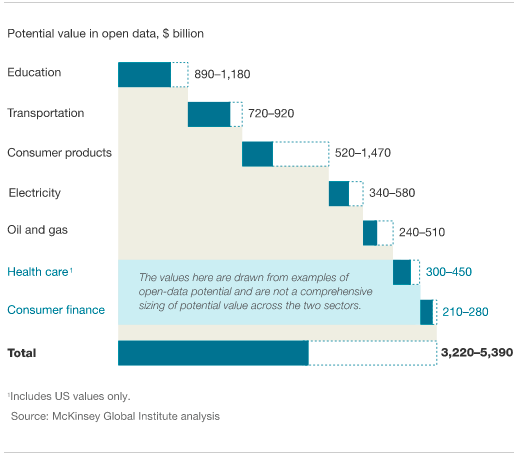
\includegraphics[width=0.8\textwidth]{Images/EstudioMckinsey}
    \caption{ Los datos abiertos pueden ayudar a generar mas de 3 billones de d�lares al a�o en el mundo.}
\end{figure}

La investigaci�n sugiere que esos siete sectores exclusivamente pudieran generar mas de 3 billones de d�lares al a�o de los cuales 1,1 bill�n corresponde a Estados Unidos, 900.000 millones a Europa y los otros 1,7 billones al resto del mundo como resultado de la utilizaci�n de datos abiertos. \\

Otro punto interesante en el estudio, revela c�mo se ha incrementado el n�mero de iniciativas de portales de datos abiertos as� como el n�mero de conjuntos de datos disponibles en cada portal. Por ejemplo, en 2009, el Gobierno de Estados Unidos public� los primeros 47 conjuntos de datos y avanz� r�pidamente hasta llegar a m�s de 90000 en Octubre de 2013.  El Gobierno del Reino Unido alcanza los 10000 conjuntos de datos para esa misma fecha. \\

Por su parte, M�xico se integr� a esta iniciativa en Abril de 2014 y a la fecha en Abril de 2015 cuenta con un total de 358 conjuntos de datos.\\

Estad�sticas como la anterior est� dando pie para la creaci�n de nuevos negocios y ayudando a compa��as ya establecidas a explorar nuevos segmentos de mercado, definir nuevos productos y servicios y mejorar la eficiencia y efectividad de sus operaciones.\\

A�n cuando el fen�meno de datos abiertos a�n esta en sus inicios en nuestro pa�s, podemos observar un claro potencial para utilizar la informaci�n como un instrumento para ayudar a las instituciones gubernamentales a reemplazar la toma de decisiones tradicional por un enfoque orientado a datos. El an�lisis de datos abiertos tambi�n puede ayudar a descubrir preferencias de los ciudadanos, permitiendo a las instituciones mejorar sus servicios y descubrir anomal�as y problemas. \\

Con base en esta informaci�n es que desarrollar una aplicaci�n enfocada a facilitar el proceso de b�squeda y an�lisis de los datos abiertos disponibles prueba ser de gran conveniencia y viabilidad en nuestro entorno global actual.\\ % Justificaci�n
\chapter{Bases Te�ricas} 

\section{Marco Historico y Contextual}

El t�rmino datos abiertos apareci� por primera vez en 1995, en un documento de la Agencia Cient�fica Americana. Ah� se discut�a acerca de la difusi�n de informaci�n geof�sica y ambiental y promov�a una apertura de el intercambio de informaci�n cient�fica entre diferentes pa�ses como requisito para el an�lisis y la comprensi�n de �stos fen�menos globales.  \\
Pero fue hasta que los ideales cient�ficos se cruzaron con los ideales del software libre, que surgi� el concepto tal y como lo conocemos hoy en d�a. \\
En Diciembre de 2007, en Sebastopol, California, un grupo de 30 l�deres entre ellos Tim O\rq Reilly and Lawrence Lessig \cite{lathrop2010open} se reunieron para discutir y definir el concepto de datos p�blicos y abiertos as� como los principios que permiten evaluarlos. 
Los resultados hasta la fecha han excedido las expectativas. En Enero de 2009, el Presidente Barack Obama tomo el mando de los Estados Unidos de Am�rica y firm� el Memorando para la Transparencia y el Gobierno Abierto, declarando \enquote{ La informaci�n mantenida por el Gobierno Federal es un recurso nacional. Mi administraci�n tomar� las acciones apropiadas, consistentes con la ley, para difundir la informaci�n r�pidamente en formatos que el p�blico pueda r�pidamente consultar y utilizar } \cite{memorandum}\\
En Mayo de ese mismo a�o, Data.gov iniciaba operaciones con �nicamente 47 conjuntos de datos. Ahora, 6 a�os despu�s la plataforma contiene m�s de 100,000 conjuntos de datos de 227 agencias y organizaciones locales, estatales y federales. \\
\clearpage
Por su parte en M�xico, El 20 de septiembre de 2011, el Presidente de la Rep�blica Mexicana present� ante la Alianza para el Gobierno Abierto, el plan de acci�n de M�xico.  \\ Los gobiernos que se incorporen a la Alianza para el Gobierno Abierto elaborar�n un Plan de Acci�n que contenga compromisos concretos.  En base a esos compromisos se lanz� el Datatron, una encuesta digital para conocer m�s sobre la demanda de Datos Abiertos y abrir el proceso a una mayor participaci�n. El Datatron ped�a a los encuestados elegir qu� datos de gobierno le gustar�a conocer. Como resultado de dicha encuesta es que surge la plataforma de Datos Abiertos del Gobierno Mexicano (\texorpdfstring{\href{http://datos.gob.mx}
                {datos.gob.mx}}
                {datos.gob.mx})  \\
Es as� que el estudio se desarrolla dentro de un contexto en donde el Movimiento Datos Abiertos ha alcanzado amplios niveles de popularidad dentro de los gobiernos regionales y nacionales.
El proyecto de intervenci�n comprende el total de 358 conjuntos de datos abiertos publicados desde Abril del 2014 a Abril del 2015 en la plataforma de Datos Abiertos del Gobierno Mexicano (\texorpdfstring{\href{http://datos.gob.mx}
                {datos.gob.mx}}
                {datos.gob.mx})   \\
                
 \begin{figure}[h!]
  \centering
    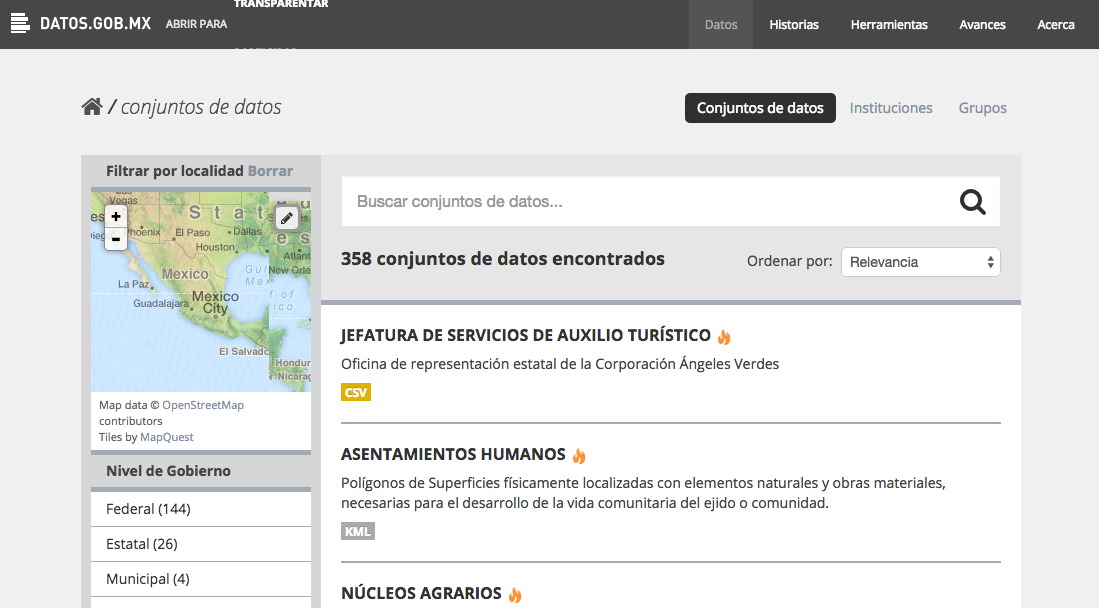
\includegraphics[width=1\textwidth]{Images/CatalogoDatosMx}
    \caption{ Cat�logo de Datos Abiertos del Gobierno de M�xico.}
\end{figure}

\clearpage

\section{Marco Referencial}

La propuesta de estudio esta fundamentada tecnol�gicamente en una librer�a de c�digo abierto para b�squeda y recuperaci�n de la informaci�n conocido como Lucene.\\
Lucene fue originalmente escrita en en lenguaje de programaci�n Java por Doug Cutting (creador tambi�n de Hadoop) en 1997. \cite{luceneinaction}
En el a�o 2000, Lucene se convirti� en una librer�a de c�digo abierto alojada en SourceForge y r�pidamente gan� adeptos por lo que en 2001 fue adoptaba por la fundaci�n Apache.
El n�mero de contribuyentes creci� sostenidamente, y a trav�s de los a�os, Lucene ha sido traducido a m�ltiples lenguajes de programaci�n, incluidos  C++, C\#, Perl, y Python.
En la versi�n original de Java o en cualquiera de sus otras versiones, Lucene es ampliamente usado en el mundo. Ejemplos de sus aplicaciones incluyen \cite{lucenepoweredby}:

\begin{enumerate}
\item Bixee - Motor de B�squeda de empleos en India.
\item Casabuscador - Motor de B�squeda para la renta y venta de bienes ra�ces en Espa�a.
\item CiteSeerX - Motor de B�squeda de documentos acad�micos. 
\item CodeCrawler - Motor de B�squeda de c�digo fuente. 
\item Dialo.de - Motor de B�squeda para el directorio de servicios secci�n amarilla para Alemania. 
\item Doctoralia - Motor de B�squeda para profesionales de la salud. 
\item Eclipse - Motor de B�squeda para la documentaci�n dentro de el entorno gr�fico (IDE) de Eclipse.
\item Keljob.com - Motor de B�squeda de curriculum vitae.
\item Twitter Trends - Motor de B�squeda para la herramienta que analiza las tendencias en Twitter. 
\end{enumerate}

\clearpage

\section{T�rminos B�sicos}

\textbf{Apache Lucene:}\\
Lucene es un software de recuperaci�n de informaci�n (IR) de c�digo abierto. Es una API flexible que permite a�adir capacidades de indexaci�n y b�squeda a cualquier sistema que se est� desarrollando.
\\
\textbf{Ara�a Web:}\\
Tambi�n conocida como Web Crawler por su t�rmino en Ingl�s es un programa que inspecciona las p�ginas web de forma met�dica y automatizada. Uno de los usos m�s frecuentes que se les da consiste en crear una copia de todas las p�ginas web visitadas para su procesado posterior por un motor de b�squeda que indexa las p�ginas proporcionando un sistema de b�squedas r�pido. 
\\
\textbf{Indexado:}\\
Acci�n de agregar una o m�s p�ginas web � documentos a las bases de datos de un buscador, para que estas aparezcan en los resultados de b�squedas de los mismos. 
\\
 % Bases Te�ricas
\chapter{Propuesta de Soluci�n} 

\section{Conjunto de Datos} % Propuesta De Soluci�n
\chapter{Implementaci�n de la Soluci�n} 
\section{Configuraci�n de Ambiente}
Para el ambiente de desarrollo es necesario instalar las herramientas descritas a continuaci�n.
\subsection{Instalaci�n de Apache Lucene}
La distribuci�n Java de Lucene consiste de m�ltiples librer�as en formato JAR.\\
Para obtener la distribuci�n binaria de Lucene es necesario seguir los siguientes pasos:
\begin{enumerate}
\item Descargar la versi�n mas reciente de la secci�n de descargas  en el sitio web de Apache Lucene. \texorpdfstring{\href{http://lucene.apache.org/core/downloads.html} {http://lucene.apache.org/core/downloads.html}} {http://lucene.apache.org/core/downloads.html} .  Para el prop�sito de este proyecto se trabaj� con la versi�n 4.9.0 
\item Extraer el archivo binario a el directorio deseado dentro del sistema.
\item Dentro de el nuevo directorio se encuentran los archivos enumerados a continuaci�n, que son los �nicos necesarios para el proyecto:
\begin{enumerate}
\item \textbf{lucene-core-4.9.0.jar}.
\item \textbf{lucene-analyzers-common-4.9.0.jar}.
\item \textbf{lucene-queryparser-4.9.0.jar}.
\end{enumerate}

Estos archivos son los que se utilizar�n para construir la aplicaci�n. Para utilizarlos es necesario incluir la ubicaci�n en la lista de librer�as de clase cuando se compilen las clases de Java.
\end{enumerate}
\clearpage 

\subsection{Instalaci�n del m�dulo de Python para acceder la API de CKAN}
La interfaz ckanapi permite acceder de manera local y remota a instancias de la plataforma CKAN para realizar operaciones masivas de datos y consultas utilizando el lenguaje de programaci�n Python. \\
Esta librer�a fue desarrollada por el desarrollador Ian Ward de Ottawa, Canada y puede ser utilizada libremente ya que esta distribuida con licencia MIT.  \cite{ckanapimodule}  \\
Como prerequisito para utilizar el m�dulo de Python ckanapi  es necesario instalar Python en el sistema y es compatible con las versiones 2 y 3. 

\begin{figure}[h!]
\begin{minted}[frame=single,
               framesep=3mm,
               xleftmargin=21pt,
               tabsize=4]{python}
{     
import ckanapi

demo = ckanapi.RemoteCKAN('http://demo.ckan.org',
    user_agent='ckanapiexample/1.0 (+http://example.com/my/website)')
groups = demo.action.group_list(id='data-explorer')
print groups
}
\end{minted}
\caption{Ejemplo de solicitud remota utilizando la librer�a ckanapi en Python} 
\end{figure}

\begin{figure}[h!]
\begin{minted}[frame=single,
               framesep=3mm,
               xleftmargin=21pt,
               tabsize=4]{js}
{     
 [u'data-explorer', u'example-group', u'geo-examples', u'skeenawild']
}
\end{minted}
\caption{Ejemplo de respuesta a solicitud remota utilizando la librer�a ckanapi en Python} 
\label{json}
\end{figure}

La librer�a ckanapi ser� utilizada para consultar la plataforma de Datos Abiertos del Gobierno Mexicano utilizando el API de CKAN a trav�s de un programa escrito en lenguaje Python y a su vez descargar los documentos abiertos que las instituciones gubernamentales han hecho disponibles.\\
Los pasos para su instalaci�n son:
\begin{enumerate}
\item Descargar la librer�a de el siguiente sitio \texorpdfstring{\href{https://github.com/ckan/ckanapi}} {https://github.com/ckan/ckanapi} {https://github.com/ckan/ckanapi}.  
\item Ejecutar el comando \emph{python setup.py install}
\end{enumerate}


\clearpage

\subsection{Instalaci�n de Apache Tika}

La herramienta Apache Tika permite la extracci�n de los metadatos e informaci�n textual de los documentos abiertos que se encuentran en m�ltiples formatos. \cite{tika}. \\
Para prop�sitos de este proyecto se utilizar� para extraer datos de archivos en formato XLM, XLS, JSON y CSV.  \\
Tika es una librer�a que contiene m�ltiples analizadores (parsers en ingl�s) por cada tipo de documento soportado. La librer�a presenta la misma API para extraer texto y metadatos de un documento independientemente de el formato, e internamente encuentra el analizador apropiado, permitiendo escribir un s�lo programa que uniformemente puede trabajar con diversos tipos de archivos. \\
La �ltima versi�n disponible es la 1.7, consiste en un archivo ejecutable en formato jar llamado \textbf{tika-app-1.7.jar } y puede ser descargada de el sitio: \\
\texorpdfstring{\href{https://tika.apache.org/download.html}} {https://tika.apache.org/download.html} {https://tika.apache.org/download.html}.   \\
Una vez descargada la herramienta, �sta puede ser ejecutada en modo l�nea de comando: \\
\centerline{\emph{cat Document.pdf | java -jar tika-app-1.7.jar -}} \\
� utilizando su interfaz gr�fica: \\
\centerline{\emph{java -jar tika-app-1.7.jar --gui}} \\
\begin{figure}[h!]
  \centering
    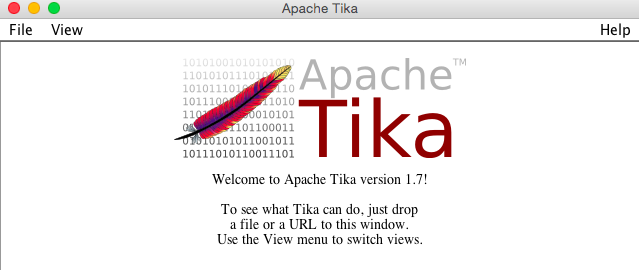
\includegraphics[width=0.8\textwidth]{Images/ApacheTika}
    \caption{ Interfaz Gr�fica de la herramienta Apache Tika.}
\end{figure}
\clearpage


\section{Detalles T�cnicos}
En las siguientes secciones se describe los detalles de implementaci�n de cada uno de los componentes involucrados en la creaci�n de la aplicaci�n. Es posible acceder al c�digo de implementaci�n en el repositorio: \\
\texorpdfstring{\href{https://github.com/citlalig/DatosAbiertosMXCrawler}} {https://github.com/citlalig/DatosAbiertosMXCrawler} {https://github.com/citlalig/DatosAbiertosMXCrawler}.   \\
\texorpdfstring{\href{https://github.com/citlalig/DatosAbiertosMXSearcher}} {https://github.com/citlalig/DatosAbiertosMXSearcher} {https://github.com/citlalig/DatosAbiertosMXSearcher}.  


\subsection{Adquirir Contenido}

El primer paso es adquirir el contenido que necesita ser indexado. Este proceso require el uso de un programa que inspecciona las p�ginas web de forma met�dica y automatizada. Dicha funcionalidad no es provista por la librer�a de Lucene por lo que se ha escrito un programa en lenguaje Python en conjunto con el m�dulo ckanapi para obtener los documentos en formato original, es decir sin procesar. \\
El programa esta compuesto de :

\begin{enumerate}
\item Una clase \textbf{CkanDatosAbiertosMX} encargada de realizar la conexi�n remota a el sitio especificado como par�metro as� como realizar las invocaciones a la API de CKAN.
\item Un m�dulo llamado \textbf{test\_ckandgm.py} encargado de hacer la conexi�n a la direcci�n URL de la plataforma de Datos del Gobierno Mexicano, consultar la lista de conjuntos de datos basado en una lista de organizaciones e iterar por cada paquete y recurso dentro de una organizaci�n particular para obtener as� la direcci�n web de el recurso y descargar el documento a un repositorio local. Los documentos descargados ser�n almacenados en un directorio llamado \emph{cat�logo} relativo a la ubicaci�n donde el programa fue ejecutado.
\end{enumerate}

\clearpage

\begin{figure}[h!]
\begin{minted}[frame=single,
               framesep=3mm,
               xleftmargin=21pt,
               tabsize=4]{python}     
import ckanapi

class CkanDatosAbiertosMX:

    def __init__(self, site_name, user_agent=None):
        self.cknsite = ckanapi.RemoteCKAN(site_name,
        user_agent= user_agent)

    def getOrganizationList(self):
        # Return a list of the names of the site organizations.
        return self.cknsite.action.organization_list()

    def getOrganizationDetails(self, org):
        # Return the details of a organization
        return self.cknsite.action.organization_show(id=org)

    def getPackageList(self):
        # Return a list of the names of the site datasets (packages).
        return self.cknsite.action.package_list()

    def getPackageDetails(self, pck):
        #Return the metadata of a dataset (package) and its resources.
        return self.cknsite.action.package_show(id=pck)

    def getTagList (self):
        #Return a list of the site tags.
        return self.cknsite.action.tag_list()

    def getTagDetails(self, tag):
        #Return the details of a tag and all its datasets.
        return self.cknsite.action.show_tag(id=tag)

    def getResourceDetails(self, rsrc):
        #Return the metadata of a resource.
        return self.cknsite.action.resource_show(id=rsrc)
\end{minted}
\caption{C�digo fuente de la clase CkanDatosAbiertosMX} 
\end{figure}

\clearpage

\begin{figure}[h!]
\begin{minted}[frame=single,
               framesep=3mm,
               xleftmargin=21pt,
               tabsize=4]{python}    
# Encoding: UTF-8
__author__ = 'citlalig'

from ckandgm import CkanDatosAbiertosMX
import urllib2
import os
import httplib
import socket
import ssl
import sys

def writeFile(fileName, data):
    output = open(fileName, 'wb')
    output.write(data)
    output.close()

def downloadFile(url, path, resource_name, resource_format):
    print 'Downloading file '+ url
    try:
        response = urllib2.urlopen(url, timeout = 30)
        if resource_format == "" :
            basename = os.path.basename(url)
            resource_format = basename[basename.rfind('.')+1:]
        file_name = resource_name + '.' + resource_format.lower()
        file_name.encode("UTF-8")
        print 'Save file ' + file_name + ' to Path: ' + path
        complete_file_name = os.path.join(path, file_name)
        writeFile(complete_file_name, response.read())

    except urllib2.HTTPError, e:
        print type(e)
    except httplib.BadStatusLine, e:
        print type(e)
    except urllib2.URLError, e:
        print type(e)
    except socket.timeout as e:
        print type(e)
    except ssl.SSLError as e:
        print type(e)
    except ssl.SSLError as e:
        print type(e)
    except IOError as e:
        print type(e)

def makeDir(dirName):
    if not os.path.exists(dirName):
        os.makedirs(dirName)
\end{minted}
\caption{C�digo fuente de el m�dulo test\_ckandgm.py (Parte 1)} 
\label{testckan1}
\end{figure}

\clearpage


\begin{figure}[h!]
\begin{minted}[frame=single,
               framesep=3mm,
               xleftmargin=21pt,
               tabsize=4]{python}    
##### MAIN CODE ####

SITE_NAME = 'http://catalogo.datos.gob.mx/'
USER_AGENT = 'MXOpenDataEngine/1.0'
organizations_list = ['pemex', 'promexico', 
	'sep', 'presidencia', 'sagarpa', 
	'shcp', 'sedesol' ]
MAIN_FOLDER = 'catalogo'
SHOW_DETAILS_ACTION = 'api/3/action/organization_show?id='
datosabiertosmx = CkanDatosAbiertosMX(SITE_NAME, USER_AGENT)
makeDir(MAIN_FOLDER)
organizations = datosabiertosmx.getOrganizationList()
for org in organizations:
    print "Organization: ", org
    if org in organizations_list:
        print "Processing Organization: " + org
        org_det = datosabiertosmx.getOrganizationDetails(org)
        name = org_det['name']
        path = os.path.join(MAIN_FOLDER, name)
        makeDir(path)
        downloadFile(SITE_NAME + SHOW_DETAILS_ACTION 
        		+ name, path, name, "json")
        packages = org_det['packages']
        for package in packages:
            package_name = package['name']
            print '\n\tProcessing Package: "' +  package_name
            path = os.path.join(os.path.join(MAIN_FOLDER , 
            	name , package_name))
            makeDir(path)
            resources = package['resources']

            for resource in resources:
                print '\t\t Processing Resources '
                		+ resource['name'] + 'in package. '
                downloadFile(resource['url'], path, 
                		resource['name'], resource['format'])


\end{minted}
\caption{C�digo fuente de el m�dulo test\_ckandgm.py (Parte 2)} 
\label{testckan2}
\end{figure}

\clearpage
El programa descrito en el c�digo fuente de las im�genes \ref{testckan1} y \ref{testckan2} deber� ser ejecutado utilizando el comando \\
\centerline{\emph{python test\_ckandgm.py \textgreater resultados.log \textgreater\textgreater resultados.log}}\\
Y producir� como resultado un directorio llamado \textbf{catalogo} en la ubicaci�n donde el programa fue ejecutado con un subdirectorio por cada organizaci�n examinada. \\

\begin{figure}[h!]
  \centering
    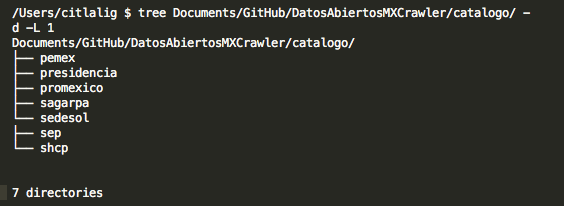
\includegraphics[width=0.8\textwidth]{Images/TreeDir}
    \caption{ Directorio de Documentos Abiertos extra�dos de una plataforma CKAN}
\end{figure}

El detalle de los resultados puede ser consultado en el Ap�ndice \ref{DocList} (Listado completo de documentos obtenidos de la plataforma datos.gob.mx)

\clearpage
\subsection{Extraer Texto}

Un paso cr�tico al construir una aplicaci�n de b�squeda es extraer texto de los documentos que se necesita indexar. En un escenario ideal, el texto deber�a de existir en formato plano, sin embargo la mayor�a de los archivos no se encuentran en tal formato, por el contrario, se encuentran en formatos populares como Word, Excel, PowerPoint, Visio, Flash, PDF, Open Office, Rich Text Format (RTF), TAR, ZIP, y BZIP2. \\
Incluso formatos relativamente sencillos como XML y HTML deben ser tratados con cuidado para no incluir accidentalmente alguna etiqueta que no forma parte del texto original. \\
Para resolver los retos que involucra el extraer texto de formatos diversos, existe la librer�a Apache Tika, la cual es una API f�cil de usar que permite filtrar texto.

El m�todo principal es \textit{parse} en la clase \textbf{org.apache.tika.parser.Parser}:

\begin{figure}[h!]
\begin{minted}[frame=single,
               framesep=3mm,
               xleftmargin=21pt,
               tabsize=4]{java}    
void parse(InputStream stream
          ContentHandler handler,
          Metadata metadata,
          ParseContext context) {}         
\end{minted}
\caption{Firma del m�todo parse en la librer�a Tika} 
\end{figure}


\begin{figure}[h!]
\begin{minted}[frame=single,
               framesep=3mm,
               xleftmargin=21pt,
               tabsize=4]{java}    
              
Metadata metadata = new Metadata();
metadata.set(Metadata.RESOURCE_NAME_KEY, f.getName());
InputStream is = new FileInputStream(f);
Parser parser = new AutoDetectParser();
ContentHandler handler = new BodyContentHandler();
ParseContext context = new ParseContext();
context.set(Parser.class, parser);
try {
	parser.parse(is, handler, metadata, new ParseContext());
} finally {
	is.close();
}
\end{minted}
\caption{Bloque de c�digo: Extraer Texto} 
\end{figure}
          
          
\clearpage
\subsection{Construir Documentos}
Una vez que hemos obtenido los archivos en su formato original, necesitan ser indexados. Para ello es necesario que su contenido sea traducido en unidades usadas por el motor de b�squeda y llamados \emph{Documentos}. \\
El  \emph{Documento} t�picamente consiste de campos con un nombre y un valor, por ejemplo: t�tulo, cuerpo, resumen, autor, url, etc. \\
Lucene provee una API para construir campos a trav�s de la clase \\ \textbf{org.apache.lucene.document.Document} pero no provee una l�gica para construir cada documento porque eso es particular de la aplicaci�n.  \\

\begin{figure}[h!]
\begin{minted}[frame=single,
               framesep=3mm,
               xleftmargin=21pt,
               tabsize=4]{java}    
              
Document doc = new Document();
doc.add(new StringField("fullpath", f.getPath(), 
	Field.Store.YES));
doc.add(new StringField("filename", f.getCanonicalPath(), 
	Field.Store.YES));
doc.add(new LongField("modified", f.lastModified(), 
	Field.Store.NO));
doc.add(new TextField("contents", handler.toString(), 
	Field.Store.NO));
\end{minted}
\caption{Bloque de c�digo: Construir un Documento} 
\end{figure}


\clearpage

\subsection{Analizar los Documentos}
Durante el proceso de analizar un documento el texto debe ser dividido en elementos llamados \emph{tokens}.  Cada \emph{token} corresponde generalmente a una palabra. \\
Lucene provee un conjunto de analizadores que permiten tener control sobre este proceso. \\
La aplicaci�n de b�squeda descrita en este documento utiliza la clase \\ \textbf{org.apache.lucene.analysis.standard.StandardAnalyzer} \\

\begin{figure}[h!]
\begin{minted}[frame=single,
               framesep=3mm,
               xleftmargin=21pt,
               tabsize=4]{java}    
              
Directory dir = FSDirectory.open(new File(indexDir));
Analyzer analyzer = new StandardAnalyzer(Version.LUCENE_4_9);
IndexWriterConfig iwc = new IndexWriterConfig(Version.LUCENE_4_9,
		analyzer);
\end{minted}
\caption{Bloque de c�digo: Analizar un Documento} 
\end{figure}

\clearpage

\subsection{Indexar los Documentos}
Durante el indexado de los documentos, el \emph{Documento} se a�ade a el \emph{�ndice}. \\
Lucene provee las herramientas necesarias para realizar este proceso utilizando la clase \\
 \textbf{org.apache.lucene.index.IndexWriter} \\

\begin{figure}[h!]
\begin{minted}[frame=single,
               framesep=3mm,
               xleftmargin=21pt,
               tabsize=4]{java}    

private IndexWriter writer = new IndexWriter(dir, iwc);

private void indexFile(File f) throws Exception {
	System.out.println("Indexing " + f.getCanonicalPath());
	Document doc = getDocument(f);
	writer.addDocument(doc);
}

public int index(String dataDir, FileFilter filter) 
	throws Exception {
	File[] files = new File(dataDir).listFiles();
	for (File f : files) {
		if (!f.isDirectory() && !f.isHidden() && f.exists() 
			&& f.canRead()
			&& (filter == null || filter.accept(f))) {
				indexFile(f);
		}
	}
	return writer.numDocs();
}

\end{minted}
\caption{Bloque de c�digo: Indexar un Documento} 
\end{figure}

\clearpage

\subsection{Construir Consulta}
Cuando se solicita una consulta, la solicitud original se traduce a un objeto de tipo \emph{Query}. Los objetos \emph{Query} pueden ser simples o complejos. Lucene provee un paquete llamado \emph{QueryParser} para convertir texto a objetos \emph{Query} utilizando las clases:\\
\textbf{org.apache.lucene.queryparser.classic.QueryParser} y \\
\textbf{org.apache.lucene.search.Query} \\

\begin{figure}[h!]
\begin{minted}[frame=single,
               framesep=3mm,
               xleftmargin=21pt,
               tabsize=4]{java}    
Analyzer analyzer = new StandardAnalyzer(Version.LUCENE_4_9);
QueryParser parser = new QueryParser(Version.LUCENE_4_9, "contents",
	analyzer);
Query query = parser.parse(q);
\end{minted}
\caption{Bloque de c�digo: Construir Consulta} 
\end{figure}

\clearpage

\subsection{Ejecutar Consulta}
La ejecuci�n de una consulta es el proceso de consultar el \emph{�ndice} y regresar los \emph{Documentos} que concuerdan.\\
La clase para ejecutar la consulta es \textbf{org.apache.lucene.search.IndexSearcher} \\ 
\begin{figure}[h!]
\begin{minted}[frame=single,
               framesep=3mm,
               xleftmargin=21pt,
               tabsize=4]{java}    

IndexSearcher is = new IndexSearcher(reader);
long start = System.currentTimeMillis();
TopDocs hits = is.search(query, 10);
long end = System.currentTimeMillis();

System.err.println("Found " + hits.totalHits + " document(s) (in "
+ (end - start) + " milliseconds) that matched query '" + q
+ "':");

\end{minted}
\caption{Bloque de c�digo: Ejecutar Consulta} 
\end{figure}

\clearpage

\subsection{Mostrar Resultados}
Una vez que se obtienen los \emph{Documentos} que concuerdan con una consulta, y han sido ordenados, est�n listos para ser mostrados de una manera que sea intuitiva para el usuario. A su vez, la interfaz deber� permitir b�squedas adicionas o filtrado de b�squeda.  Lucene se encarga de administrar este proceso pero permitiendo personalizar los resultados.  \\

\begin{figure}[h!]
\begin{minted}[frame=single,
               framesep=3mm,
               xleftmargin=21pt,
               tabsize=4]{java}    

for (ScoreDoc scoreDoc : hits.scoreDocs) {
	Document doc = is.doc(scoreDoc.doc);
	System.out.println(doc.get("fullpath"));
}
\end{minted}
\caption{Bloque de c�digo: Mostrar Resultados} 
\end{figure}

 % Implementaci�n
\chapter{Resultados Obtenidos} 

En esta secci�n se demuestra como una vez que los archivos han sido adquiridos a trav�s de la plataforma CKAN, es sencillo realizar el Indexado y B�squeda de texto dentro de el contenido y metadatos de un documento mediante el programa que fue escrito  para ese prop�sito utilizando las clases que la herramienta Apache Lucene provee.

\section{Resultados de la ejecuci�n del proceso de Indexado}

Los comandos necesarios para ejecutar la clase TikaIndexer.java y por lo tanto iniciar el proceso de Indexado se describen a continuaci�n. \\ 
Se ejecutar� una vez por cada subdirectorio correspondiente a una instituci�n gubernamental para mayor claridad: \\
\emph{Usage: java datos.gob.mx.TikaIndexer <index dir> <data dir>} \\
\begin{figure}[h!]
\begin{minted}[frame=single,
               framesep=3mm,
               xleftmargin=21pt,
               tabsize=4]{bash}
java -cp $LUCENE_HOME/core/lucene-core-4.9.0.jar:\
	$LUCENE_HOME/analysis/common/lucene-analyzers-common-4.9.0.jar:\
	$APP_HOME/bin:\
	$LUCENE_HOME/core/tika-app-1.7.jar\
	datos.gob.mx.TikaIndexer index  $DATA_CATALOG/catalogo/pemex
\end{minted}
\caption{Ejecutar la clase TikaIndexer.java} 
\label{bash}
\end{figure}
\clearpage
Y el resultado de la ejecuci�n ser�n los Documentos indexados en el directorio indicado. 
\begin{figure}[h!]
\begin{minted}[frame=single,
               framesep=3mm,
               xleftmargin=21pt,
               tabsize=4]{bash}
Indexing pemex/pr-elaboracion-de-petroliferos/
	PR-Elaboracion de petroliferos.csv
Indexing pemex/pr-elaboracion-de-petroliferos/
	PR-Elaboracion de petroliferos.xml
Indexing pemex/pr-elaboracion-de-petroliferos-por-refineria/
	PR-Elaboracion de petroliferos por refineria.csv
Indexing pemex/pr-elaboracion-de-petroliferos-por-refineria/
	PR-Elaboracion de petroliferos por refineria.xml
Indexing pemex/pr-estructura-de-precios-de-gasolinas-y-diesel/
	PR-Estructura de precios de gasolinas y diesel.csv
Indexing pemex/pr-estructura-de-precios-de-gasolinas-y-diesel/
	PR-Estructura de precios de gasolinas y diesel.xml
Indexing pemex/pr-proceso-de-crudo/
	PR-Proceso de crudo.csv
Indexing pemex/pr-proceso-de-crudo/
	PR-Proceso de crudo.xml
Indexing pemex/pr-valor-comercio-exterior/
	PR-Valor comercio exterior.csv
Indexing pemex/pr-valor-comercio-exterior/
	PR-Valor comercio exterior.xml
Indexing pemex/pr-valor-ventas/
	PR-Valor ventas.csv
Indexing pemex/pr-valor-ventas/
	PR-Valor ventas.xml
Indexing pr-volumen-comercio-exterior/
	PR-Volumen comercio exterior.csv
Indexing pemex/pr-volumen-comercio-exterior/
	PR-Volumen comercio exterior.xml
Indexing pemex/pr-volumen-ventas/
	PR-Volumen ventas.csv
Indexing pemex/pr-volumen-ventas/
	PR-Volumen ventas.xml
Indexing pemex/quejas-oic-junio-2014/
	Petroleos Mexicanos y Organismos Subsidiarios.csv
Indexing pemex/quejas-oic-septiembre-2014/
	Petroleos Mexicanos y Organismos Subsidiarios.csv
Indexing 181 files took 3583 milliseconds
\end{minted}
\caption{ Crear �ndices de los archivos existentes en un directorio.}
\label{bash}
\end{figure}

\clearpage
\section{Resultados de la ejecuci�n del proceso de B�squeda}
Los comandos necesarios para ejecutar la clase Searcher.java y por lo tanto realizar una b�squeda a partir de los �ndices existentes se describen a continuaci�n: \\
\emph{Usage: java datos.gob.mx.Searcher <index dir> <query>} \\
\begin{figure}[h!]
\begin{minted}[frame=single,
               framesep=3mm,
               xleftmargin=21pt,
               tabsize=4]{bash}
java -cp $LUCENE_HOME/core/lucene-core-4.9.0.jar:\
	$LUCENE_HOME/analysis/common/lucene-analyzers-common-4.9.0.jar:\
	$APP_HOME/bin:\
	$LUCENE_HOME/queryparser/lucene-queryparser-4.9.0.jar\
	datos.gob.mx.Searcher index pemex
\end{minted}
\caption{Ejecutar la clase Searcher.java} 
\label{bash}
\end{figure}

\begin{figure}[h!]
\begin{minted}[frame=single,
               framesep=3mm,
               xleftmargin=21pt,
               tabsize=4]{bash}
Found 210 document(s) (in 37 milliseconds) 
	that matched query 'pemex':
catalogo/pemex/quejas-oic-junio-2014/
	Petroleos Mexicanos y Organismos Subsidiarios.csv
catalogo/pemex/quejas-oic-septiembre-2014/
	Petroleos Mexicanos y Organismos Subsidiarios.csv
catalogo/pemex/pemex.json
catalogo/pemex/pemex-estadisticas-seleccionadas/
	PEMEX Estadisticas seleccionadas.xml
\end{minted}
\caption{ Resultados de B�squeda. Query = pemex}
\label{pemexq}
\end{figure}
El resultado de la ejecuci�n ser�n la lista de Documentos que satisfacen la consulta. \\ La consulta mostrada previamente es muy sencilla sin embargo pueden ser tan complicadas como se desee. \\
Un ejemplo mas elaborado de b�squeda utilizando una expresi�n de consulta utilizando metadatos, basado en contenido, titulo, y fecha de modificaci�n se muestra a continuaci�n: \\

\begin{figure}[h!]
\begin{minted}[frame=single,
               framesep=3mm,
               xleftmargin=21pt,
               tabsize=4]{bash}
$ java -cp $LUCENE_HOME/core/lucene-core-4.9.0.jar:\
	$LUCENE_HOME/analysis/common/lucene-analyzers-common-4.9.0.jar:\
	$APP_HOME/bin:\
	$LUCENE_HOME/queryparser/lucene-queryparser-4.9.0.jar \
	datos.gob.mx.Searcher index 
	"indicadores+pobreza modified:[1/1/15 TO 12/31/15]
	 -multidimensional"
Found 7 document(s) (in 88 milliseconds) 
that matched query 'indicadores+pobreza 
	modified:[1/1/15 TO 12/31/15] -multidimensional':
catalogo/presidencia/
	mexico-incluyente-indicadores-del-pnd-y-pmp/
	Indicadores del Plan Nacional de Desarrollo, 2013-2018 2. 
	M�xico Incluyente.xlsx
catalogo/presidencia/mexico-con-educacion-de-calidad-
	indicadores-del-pnd-y-pmp/
	Indicadores del Programa Nacional de Cultura F�sica 
	y Deporte 2014-2018 
	y su vinculaci�n con la planeaci�n nacional.xlsx
catalogo/presidencia/mexico-con-educacion-de-calidad-
	indicadores-del-pnd-y-pmp/
	Indicadores del Plan Nacional de Desarrollo, 
	2013-2018 3. 
	M�xico con Educaci�n de Calidad.xlsx
catalogo/presidencia/mexico-incluyente-estadisticas-nacionales/
	Indicadores de seguridad social del IMSS 
	Concepto.xlsx
catalogo/presidencia/mexico-con-educacion-de-calidad-
	indicadores-del-pnd-y-pmp/
	Indicadores del Programa Sectorial de 
	Educaci�n 2013-2018 
	y su vinculaci�n con la planeaci�n nacional 
	(Ciclos escolares).xlsx
catalogo/presidencia/mexico-en-paz-indicadores-del-pnd-y-pmp/
	Indicadores del Programa Sectorial de Defensa Nacional 2013-2018 
	y su vinculaci�n con la planeaci�n nacional.xlsx
catalogo/presidencia/mexico-incluyente-indicadores-del-pnd-y-pmp/
	Indicadores del Programa Nacional para el Desarrollo 
	y la Inclusi�n de las Personas con Discapacidad, 2014-2018 
	y su vinculaci�n con la planeaci�n nacional.xlsx
\end{minted}
\caption{ Ejemplo de B�squeda. Query = 'indicadores+pobreza modified:[1/1/15 TO 12/31/15] -multidimensional':}
\label{pemexq}
\end{figure}





 % Resultados


%% ----------------------------------------------------------------
% Now begin the Appendices, including them as separate files

%\addtocontents{toc}{\vspace{2em}} % Add a gap in the Contents, for aesthetics

\appendix % Cue to tell LaTeX that the following 'chapters' are Appendices
\chapter{Resumen de formatos de archivos m�s comunes}


\textbf{JSON} \\  Acr�nimo de JavaScript Object Notation, es un formato ligero para el intercambio de datos. JSON es un subconjunto de la notaci�n literal de objetos de JavaScript que no requiere el uso de XML.\\
\textbf{XML} \\ Siglas en ingl�s de eXtensible Markup Language ('lenguaje de marcas extensible'), es un lenguaje de marcas desarrollado por el World Wide Web Consortium (W3C) utilizado para almacenar datos en forma legible. \\
\textbf{XLS} \\ La extensi�n de archivo por defecto para aplicaciones de hojas de c�lculo. \\
\textbf{CSV} \\ Tipo de documento en formato abierto sencillo para representar datos en forma de tabla, en las que las columnas se separan por comas y las filas por saltos de l�nea.  \\
\textbf{TXT} \\La extensi�n para archivo compuesto �nicamente por texto sin formato, s�lo caracteres, lo que lo hace tambi�n legible por humanos.  \\
\textbf{ZIP} \\Formato de compresi�n sin p�rdida, muy utilizado para la compresi�n de datos como documentos, im�genes o programas. \\
\textbf{KMZ} \\ Es un lenguaje de marcado basado en XML para representar datos geogr�ficos en tres dimensiones en formato comprimido.  \\ % Appendix Title
\lhead{\emph{Ejemplos de Implementaciones CKAN en el mundo}}
\chapter{Ejemplos de implementaciones CKAN en el mundo}
 \centering
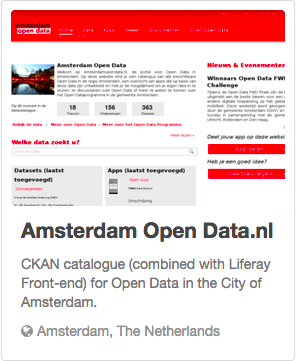
\includegraphics{Images/AmsterdamOpenData} \\
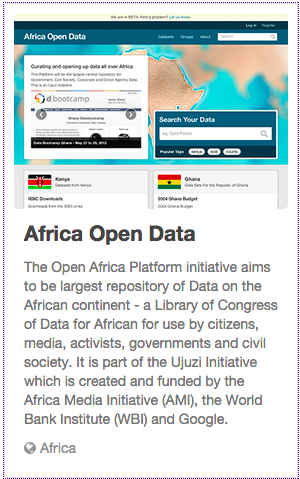
\includegraphics{Images/AfricaOpenData} \\
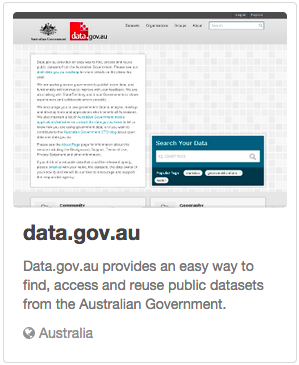
\includegraphics{Images/AustraliaOpenData} \\
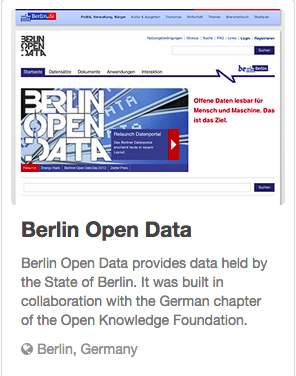
\includegraphics{Images/BerlinOpenData} \\
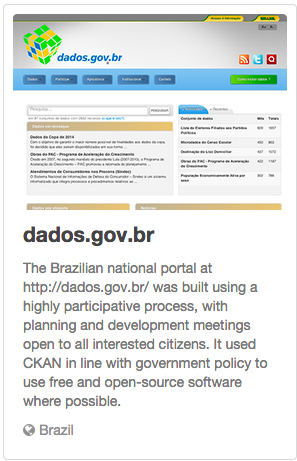
\includegraphics{Images/BrasilOpenData} \\
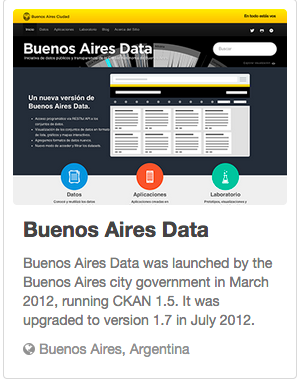
\includegraphics{Images/BuenosAiresOpenData} \\
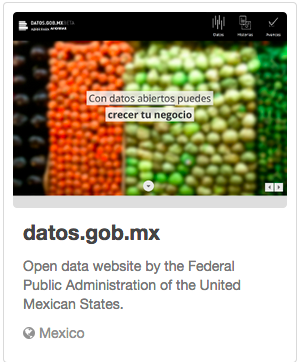
\includegraphics{Images/MexicoOpenData} \\
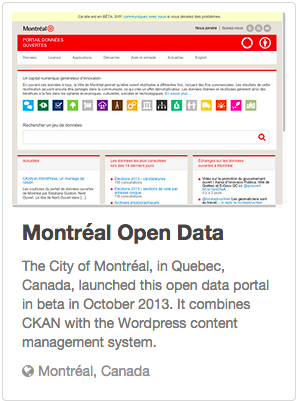
\includegraphics{Images/MontrealOpenData} \\
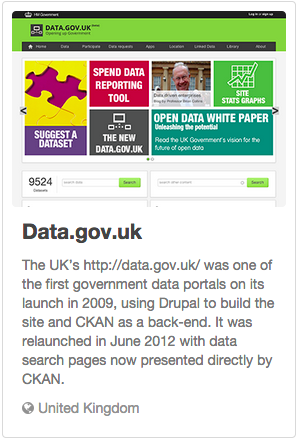
\includegraphics{Images/UKOpenData} \\
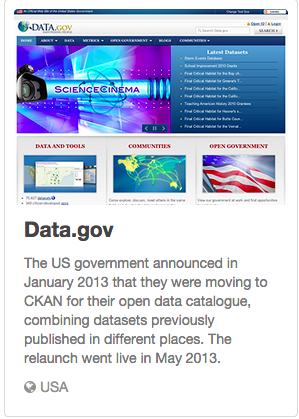
\includegraphics{Images/USOpenData} \\

	% Appendix Title
\chapter{Calendario de Actividades} 	% Appendix Title
%\input{Appendices/AppendixC} % Appendix Title

%\addtocontents{toc}{\vspace{2em}}  % Add a gap in the Contents, for aesthetics
\backmatter

%% ----------------------------------------------------------------
\label{Bibliography}
\lhead{\emph{Bibliography}}  % Change the left side page header to "Bibliography"
\bibliographystyle{unsrtnat}  % Use the "unsrtnat" BibTeX style for formatting the Bibliography
\bibliography{Bibliography}  % The references (bibliography) information are stored in the file named "Bibliography.bib"

\end{document}  % The End
%% ----------------------------------------------------------------